\chapter[Conclusão]{Conclusão}

Nesse estudo foi desenvolvido um Sistema de Comunicação Interveicular para Alerta
de Colisões em Rodovias (CIAC). O objetivo desse projeto foi elaborar um dispositivo
capaz de alertar ao condutor do veículo se a ultrapassagem é ou não segura, de
forma ágil e precisa. Para que o sistema funcione é necessário que todos os
carros próximos ao veículo com intenção de ultrapassar obtenham o sistema
interveicular. Somente assim, a adoção do sistema apresenta-se como uma
ferramenta apta a colaborar com a diminuição de acidentes em rodovias de
mão dupla.

Além disso, o sistema deverá ser ativado ao dar partida no veículo e só
 poderá ser utilizado em veículos automotores, com exceção de veículos
 motorizados de duas ou três rodas. O seu funcionamento é baseado na
 comunicação interveicular composta principalmente por GPS, transponder,
 Lidar, Radar, sensor de rotação e câmera. Esses dispositivos foram escolhidos
 de forma criteriosa, conforme analisado no presente relatório, para que o
 sistema funcione corretamente perante algumas adversidades do clima e do
 relevo local.

A intenção de ultrapassagem é identificada em quatro etapas, sendo elas: O
acionamento da seta, mudança na angulação do volante, mudança de faixa e aumento
da proximidade entre dois carros na mesma faixa. Após detectar a intenção de
realizar a ultrapassagem o sistema calcula se há um outro veículo em movimento
no sentido oposto.

O esquema a seguir representa, de forma resumida, como é a interação entre o
motorista e o sistema.

\begin{figure}[h]
  \centering
  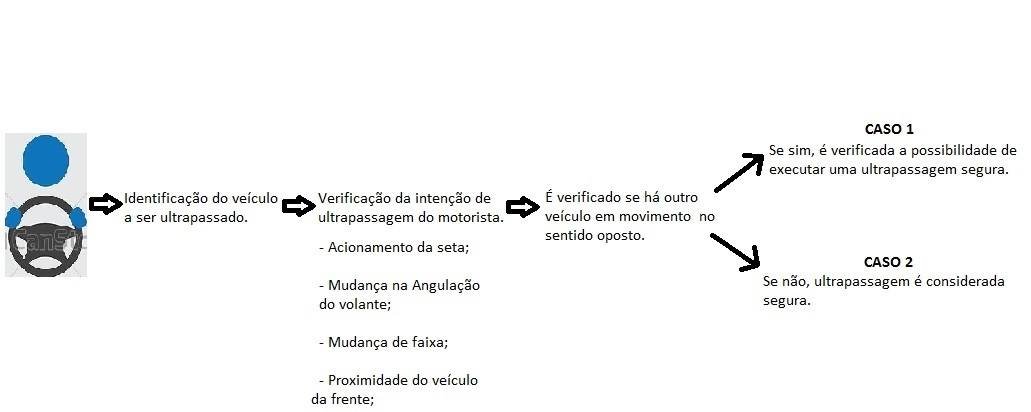
\includegraphics[width=400px, scale=1]{figuras/funcionamentociac}
  \caption{Esquema do funcionamento do CIAC}
\label{fig:funcionamentociac}
\end{figure}

\begin{figure}[h]
  \centering
  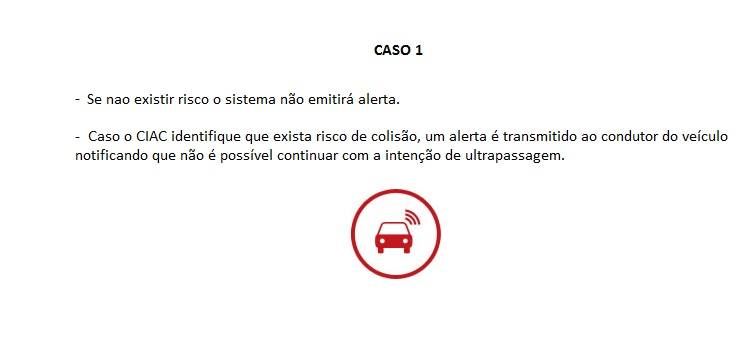
\includegraphics[width=400px, scale=1]{figuras/funcionamentociac1}
  \caption{Funcionamento do sistema de acordo com o caso 1}
\label{fig:funcionamentociac1}
\end{figure}

Com a utilização do CIAC, espera-se que o número de acidentes frontais em rodovias
brasileiras diminua consideravelmente e que o sistema desenvolvido proporcione
segurança para o motorista ao realizar uma ultrapassagem em trechos de pouca
visibilidade, por exemplo. O dispositivo funcionará ininterruptamente, dessa
forma sempre que for detectada a intenção de ultrapassagem o CIAC indicará se é
possível ou não seguir com a manobra. Tudo isso de forma rápida e eficiente,
facilitando então a interação entre o homem e a máquina.
